% !TEX TS-program = pdflatexmk
% !BIB TS-program = bibtex

\documentclass[12pt, a4paper, oneside]{book}
\usepackage{import}
\subimport{../}{preamble}
\ExecuteBibliographyOptions{articletitle=false}
\standalonetrue
\onehalfspacing
\begin{document}

\begin{singlespace}
{\color{white}
\chapter{Theoretical Background}}
\label{ch:theory}
\end{singlespace}

\AddToShipoutPictureBG*{ \AtPageUpperLeft{
%{\includegraphics[width=\paperwidth, clip=true, trim=0 100 0 100]{data/chapter_cover.png}}
\put(0,-220) {\includegraphics[width=\paperwidth]{../chapter_covers/theory_cover2.png}}
\put(0,-220) {\includegraphics[width=\paperwidth]{../chapter_covers/theory_cover.png}}
\put(110,-5) {\begin{minipage}[t]{0.5\textwidth}\centering\singlespace\fontsize{9pt}{1em}\selectfont\color{white} Illustrations of nanoparticle, tip and spherical tip plasmons and the concepts of plasmon coupling and field localisation.\end{minipage}}
\put(345,-116) {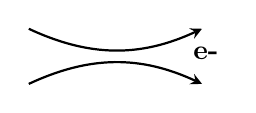
\begin{tikzpicture}[->, >=stealth, thick]
\draw (0,0.35cm) [out=-25, in=-155] to  (2.2cm,0.35cm);
\draw (0,-0.35cm) [out=25, in=155] to  (2.2cm,-0.35cm);
\node at (2.25cm,0.04cm) {\color{black}\bfseries\fontsize{13pt}{1em}\ce{e-}};
\end{tikzpicture}}
}}

As previously stated, light can be confined below the diffraction limit by exploiting plasmons. Transferring energy from a diffraction-limited photonic field into collective oscillations of conduction electrons enhances the electric field on the surface of a metallic nanostructure with nanoscale localisation. It is through the understanding and application of this phenomenon that nano-optics and sub-wavelength confinement is made possible.
This chapter deals firstly with a theoretical description of electromagnetic fields and the optical properties of metals. From this basis the concept of a plasmon can be introduced and the different kinds of plasmons defined, illustrating how they interact within different spatial regimes. Through this behaviour, the study of charge transfer in plasmonic systems, specifically quantum charge transport, is addressed. Finally, the plasmonics of metallic tips is discussed in preparation for the experiments described in later chapters studying plasmon interaction through each of the characteristic spatial regimes.

\subimport{./}{plasmons}
\subimport{./}{plasmon_coupling}

% How is the tip experiment different to static systems
Although charge transfer effects have been shown in previous reports by varying the conductivity of a fixed gap, there has yet to be a report showing the optical response of a dynamic dimer structure correlated with its electronic response. It is the aim of this project to successfully determine the relationship between electronic and plasmonic phenomena using a dual plasmonic nano-tip dimer. Metallic nano-tips are a plasmonic geometry currently receiving significant attention from the plasmonics community. In order to use nano-tips to determine the effects of quantum charge transfer on plasmonics, their supported plasmons must first be described.

\subimport{./}{tip_plasmonics_literature}

\section{Conclusions}

The coupling of plasmons in metallic nanostructures is now widely exploited in order to enhance and confine optical fields on nanometric scales. In order to maximise enhancement, the characteristic scales of these gap structures are rapidly approaching the sub-nm level where quantum mechanics can no longer be ignored. As recent results have shown, charge transfer in such small gaps can lead to the emergence of new plasmonic phenomena and a break down of classical field confinement. This regime must therefore be well understood if the characteristic size of plasmonic devices are to continue decreasing.

The effects of electron tunnelling and charge transfer in sub-nm plasmonic gaps have only been touched upon in recent years and still require significant investigation. To this extent, tips whose plasmons readily couple with light provide a useful platform for dynamically studying the fundamental plasmonics of nanogaps. Their well-developed experimental geometries for topological measurements form the basis of microscopes integrating optics and tip-based surface techniques. By using such a setup, quantum effects in coupled plasmonic systems can be further investigated by controllably reducing a gap into the sub-nm regime.

To date there have been no direct correlated measurements between plasmon resonances and quantum transport effects. Tunnelling has been inferred from direct measurements of plasmon resonances without electronic measurements \cite{savage2012, scholl2013} and from variables influenced by the gap field enhancement, which in some cases provide electronic measurements \cite{tan2014, zhu2014, hajisalem2014, cha2014}. The effects of quantum charge transport can be better understood with correlated electrical and force measurements. By using an experimental geometry related to AFM these measurements become possible.

\ifstandalone
\begin{singlespace}
\fontsize{8pt}{1em}\selectfont
\printbibliography[notcategory=fullcited]
\end{singlespace}
\fi

\end{document}